\documentclass[sigconf,anonymous,review]{acmart}
\usepackage{booktabs}
\usepackage{amsmath}
\usepackage{graphicx}
\usepackage{algorithm}
\usepackage{algpseudocode}
\usepackage{tikz}
\usetikzlibrary{arrows.meta,positioning,fit}
\bibliographystyle{ACM-Reference-Format}
\setlength{\emergencystretch}{1em}

\title{When May an Agent Claim Success? Verification Contracts for Open-World Outcomes}
\author{Anonymous Authors}
\keywords{AI agents, verification, selective prediction, auditability, open-world outcomes}
\ccsdesc[500]{Computing methodologies~Intelligent agents}
\ccsdesc[300]{Software and its engineering~Software verification}

\begin{document}
\begin{abstract}
Agent systems increasingly convert uncertain observations into consequential state transitions: releasing payment, marking work complete, granting access, or advancing a workflow. When an outcome is represented by a screenshot, image, document, link, or contextual claim, evaluator accuracy alone does not establish that a system is entitled to act. The governing rule may have changed after submission, evidence may be replayed from another task, uncertainty may be coerced into a binary decision, or the resulting transition may be impossible to reconstruct. We introduce the \emph{Verification Contract}, a protocol abstraction that commits before submission to an intent, proof obligations, an evidence-binding function, a selective verifier, admissible transitions, and a receipt reconstruction function. We define four measurable properties---ex-ante consistency, evidence binding, selective safety, and decision reconstructability---and instantiate them in a contract-governed verifier. We further introduce JOVE-Core, a grouped benchmark of digital outcomes and matched property violations. The preregistered primary endpoint is unsafe positive transition rate at a fixed automation-coverage floor. The paper asks a systems question stricter than whether evidence appears plausible: under what declared conditions is the result protocol-eligible for downstream reliance?
\end{abstract}
\maketitle

\section{Introduction}
Autonomous agents publish content, change account settings, submit documents, coordinate people, and initiate transfers. The terminal condition of such workflows is frequently represented by evidence rather than authoritative state. A downstream application must convert an uncertain observation into a discrete consequence: payment is released or withheld; access is granted or denied; a workflow advances or stops.

A learned evaluator may judge that evidence ``looks correct'' while the surrounding system remains unsafe to act. The acceptance rule may have been selected after evidence arrived. A semantically correct screenshot may belong to another task or policy version. A model provider may have failed. Several evaluators may share a blind spot. A stored PASS flag may reveal neither the decisive obligation nor why automation was permitted. These failures concern not only classification, but the protocol conditions under which a classification controls state.

We propose a \emph{Verification Contract}: an ex-ante, machine-readable agreement among requester, evidence producer, verifier, and downstream consumer. It defines what is claimed, what evidence is required, how evidence is bound to the claim, how uncertainty is handled, which transitions are admissible, and what receipt must exist afterward. The contract governs the entire path from intent to consequence rather than only the model judgment in the middle.

Our contributions are: (1) a protocol abstraction for authorizing deterministic transitions from probabilistic observations; (2) four independently measurable contract properties; (3) an executable prototype with explicit trust boundaries and three-valued authorization semantics; and (4) JOVE-Core, a property-centered evaluation with matched defects, grouped splits, held-out task classes, and a preregistered risk-at-coverage endpoint.

The claim is intentionally narrower than universal truth verification. We test whether explicit and enforceable authorization predicates prevent unsafe transitions that aggregate judge accuracy cannot distinguish. The claim is falsified if the complete contract fails the frozen coverage floor, does not reduce unsafe transitions relative to a strong policy-aware judge, or fails to transfer to held-out task classes.

\section{Related Work and Novelty Boundary}
\sloppy
\paragraph{Contracts and formal checking.} Software contracts specify preconditions, postconditions, and invariants over machine-observable state \cite{meyer1997object}. Proof-carrying code couples an executable with a machine-checkable proof \cite{necula1997proof}. Runtime verification monitors traces against formal properties \cite{leucker2009brief}. Open-world evidence differs because the postcondition itself is inferred from incomplete and manipulable observations. We borrow the producer--checker--policy separation but do not claim semantic soundness.

\paragraph{Selective prediction and model judges.} Selective prediction permits rejection to control risk \cite{geifman2017selective,geifman2019selectivenet,kamath2020selectiveqa,hendrickx2024reject}. LLM-as-a-Judge studies evaluator agreement and bias \cite{zheng2023judging,liu2023geval,wang2024fair}. Both center the decision function. A calibrated evaluator can still authorize an unsafe transition if policy changes after submission, evidence is replayed, or downstream software maps errors to success.

\paragraph{Forensics, provenance, and records.} Media forensics surfaces manipulation signals but does not establish task sufficiency \cite{verdoliva2020media}. Provenance and logs support traceability but do not identify the rule that made a transition action-eligible. Verification Contracts compose such evidence under predeclared obligations and require a receipt optimized for independent reconstruction.

\paragraph{Agent evaluation and research documentation.} Agent benchmarks test increasingly consequential workflows \cite{liu2023agentbench,zhou2023webarena,xie2024osworld,xu2024theagentcompany}, but outcome checking is commonly embedded in task-specific evaluators. We isolate the authorization boundary as the object of study. Dataset and model documentation practices motivate explicit provenance, scope, and maintenance disclosures \cite{bender2018data,gebru2021datasheets,mitchell2019modelcards}; our artifact extends this discipline to contracts, controlled defects, receipts, and transitions.

No individual mechanism is claimed as new in isolation. The novelty boundary is their enforceable composition: \emph{precommitted obligations, task-bound evidence, selective authorization, and a reconstructable transition}. This composition exposes policy drift, replay, forced transition under uncertainty, and irreconstructability as separate experimental outcomes.

We do not prove that the six-field tuple is uniquely minimal. Minimality is an empirical design hypothesis: removing each property should selectively reintroduce its matched failure. Operational independence is therefore tested by ablation rather than asserted from syntax. Likewise, the paper applies established three-valued logic at the agent authorization boundary; it does not claim to invent that logic.
\fussy

\section{Verification Contracts}
Let workflow state be $s\in\mathcal{S}$ and let $a^+$ denote a consequential positive transition. A Verification Contract is
\begin{equation}
K=\langle I,P,B,V,A,R\rangle,
\end{equation}
where $I$ is declared intent and immutable constraints; $P$ is a set of ex-ante proof obligations; $B$ binds evidence to task, policy version, and context; $V$ is a selective verifier; $A$ defines admissible state transitions; and $R$ reconstructs a receipt.

Each authorization predicate evaluates in $\{\top,\bot,?\}$. Unknown is never truthy. Under strong Kleene conjunction, a positive transition is authorized only when
\begin{align}
\mathrm{Authorize}(K,e,o,h,a^+) ={}& \mathrm{Stable}(P)\land \mathrm{Bound}(B,e) \notag\\
&\land \mathrm{Accepted}(V,K,e,o,h) \notag\\
&\land \mathrm{Reconstructable}(R).
\end{align}
evaluates to $\top$. Any $\bot$ blocks the transition; any $? $ produces abstention.

This semantics separates three states that binary judges often collapse. A known failed obligation is a rejection: the submitted evidence does not satisfy the committed rule. An unresolved obligation is an abstention: the system lacks a valid basis for either acceptance or rejection. Only a fully satisfied authorization predicate is acceptance. This distinction matters operationally because a correctable submission gap, a provider outage, and a detected replay require different downstream actions even if none permits immediate settlement.

\begin{figure*}[t]
\centering
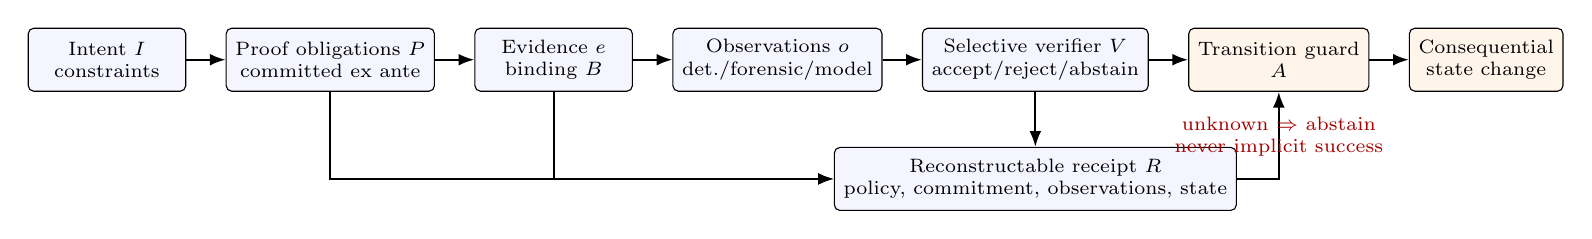
\begin{tikzpicture}[font=\scriptsize, node distance=4mm and 5mm,
box/.style={draw,rounded corners=2pt,minimum height=8mm,minimum width=20mm,align=center,fill=blue!4},
state/.style={draw,rounded corners=2pt,minimum height=8mm,minimum width=18mm,align=center,fill=orange!8},
arr/.style={-{Latex[length=2mm]},thick}]
\node[box] (intent) {Intent $I$\\constraints};
\node[box,right=of intent] (policy) {Proof obligations $P$\\committed ex ante};
\node[box,right=of policy] (evidence) {Evidence $e$\\binding $B$};
\node[box,right=of evidence] (observe) {Observations $o$\\det./forensic/model};
\node[box,right=of observe] (verify) {Selective verifier $V$\\accept/reject/abstain};
\node[state,right=of verify] (guard) {Transition guard\\$A$};
\node[state,right=of guard] (transition) {Consequential\\state change};
\draw[arr] (intent)--(policy); \draw[arr] (policy)--(evidence); \draw[arr] (evidence)--(observe); \draw[arr] (observe)--(verify); \draw[arr] (verify)--(guard); \draw[arr] (guard)--(transition);
\node[box,below=7mm of verify] (receipt) {Reconstructable receipt $R$\\policy, commitment, observations, state};
\draw[arr] (policy.south) |- (receipt.west); \draw[arr] (evidence.south) |- (receipt.west); \draw[arr] (verify.south)--(receipt.north); \draw[arr] (receipt.east) -| (guard.south);
\node[below=2mm of guard,align=center,text=red!65!black] {unknown $\Rightarrow$ abstain\\never implicit success};
\end{tikzpicture}

\caption{A Verification Contract spans evidence production, selective verification, and downstream authorization. It is not merely a judge prompt or an audit log.}
\Description{A left-to-right protocol diagram linking intent, proof obligations, bound evidence, observations, a selective verifier, a transition guard, a consequential state change, and a reconstructable receipt.}
\label{fig:architecture}
\end{figure*}

\subsection{Contract Properties}
\textbf{Ex-ante consistency} requires decision-relevant obligations to be committed before first submission. Amendments create a new immutable version and invalidate prior evidence unless an explicit reuse rule exists. \textbf{Evidence binding} requires commitments to task identity, policy version, artifact digest, and relevant context. \textbf{Selective safety} requires declared integrity conflicts, unsupported inputs, provider degradation, or uncertainty to produce abstention rather than implicit success. \textbf{Decision reconstructability} requires an independent auditor to recover the governing policy, evidence commitment, decisive observations, verifier state, and authorized transition.

\paragraph{Enforcement invariant.} If a downstream application enforces $\mathrm{Authorize}$ as a necessary precondition for every $a^+$, no positive transition can occur while a declared predicate is explicitly false. This is an interface invariant, not a theorem that evidence is truthful or complete. The present guarantee is local to one transition; compositional guarantees across long-horizon workflows remain future work.

\subsection{Versioning and Amendment}
A contract is immutable after the first evidence commitment. Legitimate policy evolution creates $K_{v+1}$ rather than mutating $K_v$. Evidence bound to $K_v$ is inadmissible under $K_{v+1}$ unless both versions contain an explicit reuse rule. This rule prevents a requester from changing a deadline, evidence modality, or acceptance criterion after observing a submission while preserving an auditable path for corrections. An amendment record identifies the initiating principal, changed obligations, reason, and whether existing evidence was invalidated.

The contract may also constrain proof burden through an artifact-count budget, retained-byte budget, and prohibited evidence fields. These constraints do not decide whether the underlying policy is fair; they provide a machine-enforceable hook for an external governance process. Appeal policy records whether an appeal is allowed, whether it stays the consequential transition, and the response window.

\subsection{Principals and Trust Boundaries}
The requester controls intent and the initial obligations but is not trusted to modify them retroactively. The evidence producer controls submitted artifacts but is not trusted for truth, freshness, uniqueness, or task membership. The verifier operator controls observation services and thresholds but is not trusted to convert unknown states into acceptance. The downstream application controls the consequential transition and must enforce the authorization guard. Auditors and contestants may reconstruct or challenge a decision without receiving unrestricted access to private evidence. These boundaries make clear that the contract redistributes trust; it does not eliminate it.

\subsection{Receipt Semantics}
Reconstructability has two levels. \emph{Syntactic reconstructability} requires required fields and commitment links to be present and resolvable. \emph{Empirical reconstructability} asks whether an independent auditor can correctly recover the policy, evidence basis, uncertainty path, and transition reason. The former is machine-checkable; the latter is measured in the audit study. A receipt is also a contestable record. Appeals append a new signed adjudication event referencing the immutable original receipt; they never rewrite the historical decision.

\section{Contract-Governed Verification}
The prototype compiles a natural-language request into versioned, typed obligations. Deterministic fallback rules preserve a valid contract when a model compiler is unavailable. Evidence bundles carry artifact hashes and context commitments. Observation modules expose schema validity, timestamps, metadata, JPEG/PNG structure, C2PA/JUMBF presence, cross-artifact consistency, and policy-conditioned multimodal judgments. Forensic features are treated as risk signals, never authenticity proofs.

\begin{algorithm}[t]
\caption{Contract-governed selective authorization}
\begin{algorithmic}[1]
\Require Contract $K$, evidence $e$, thresholds $\theta$
\If{schema invalid or required evidence missing}
  \State \Return reject with obligation codes
\EndIf
\State $b\gets B(K,e)$
\If{$b\neq\top$} \State \Return abstain or reject by declared rule \EndIf
\State $o\gets$ deterministic, forensic, and model observations
\If{hard conflict, unsupported input, or provider degradation}
  \State \Return abstain with verifier state
\EndIf
\State $d\gets V(K,e,o;\theta)$
\If{$d=accept$ and receipt is reconstructable}
  \State \Return authorize $a^+$ and emit $R$
\ElsIf{$d=reject$}
  \State \Return reject with failed obligations
\Else
  \State \Return abstain
\EndIf
\end{algorithmic}
\end{algorithm}

The receipt is not free-form rationale. It is a canonical record containing identifiers and versions, evidence commitments, per-obligation observations, thresholds, provider/degradation state, final decision, admissible transition, and settlement reference where applicable. Syntactic completeness and human reconstruction accuracy are measured separately. Appeals reference the immutable receipt and add a new adjudication event rather than rewriting history.

The reference validator serves as a conformance oracle for contract and receipt semantics; it is not proof that every deployment path invokes the guard atomically. A conforming integration binds the receipt and consequential transition to the same immutable decision identifier, preventing a later or unrelated decision from being substituted between verification and settlement. Digital signatures can harden this linkage but are not part of the present guarantee.

\subsection{Proof-Obligation Compilation}
Natural-language requests are underspecified interfaces. The compiler maps a request to typed obligations specifying required modality, quantity, capture preference, timing, mandatory status, and decision method. Compilation follows three constraints. \emph{Intent preservation} prevents a convenient proxy from replacing the requested outcome. \emph{Minimal sufficiency} avoids collecting evidence unrelated to the decision. \emph{Decision relevance} requires every requested field to support an explicit rule. A model-assisted path proposes the structure, while deterministic fallback templates ensure that provider unavailability does not silently remove the policy boundary. In both paths the serialized contract is versioned and committed before evidence submission.

\subsection{Evidence Binding and Observation Layers}
Binding commits each artifact to a contract identifier, task identifier, policy version, server receipt time, and content digest. Optional context commitments may include a declared account, URL origin, or capture window. Hashes establish artifact identity, not authenticity. The observation layer then produces three families of evidence: deterministic schema and policy checks; forensic risk observations such as metadata, container structure, editing history signals, and C2PA/JUMBF presence; and policy-conditioned multimodal judgments. Deterministic failures dominate semantic acceptance. Forensic signals can raise risk or require review but do not independently prove fraud. Model judgments are emitted per obligation to prevent a globally plausible artifact from hiding a local failure.

\subsection{Degradation and Selective Decision}
The verifier records provider identity, model version, response validity, latency, and disagreement. Unsupported mandatory input, missing providers, malformed output, declared integrity conflicts, or disagreement beyond a frozen threshold produce unknown and therefore abstention. A degraded ensemble uses a stricter threshold rather than preserving nominal behavior. This policy prevents availability failures from being interpreted as evidence against the submitter or, more dangerously, as implicit permission to settle.

\subsection{Implementation Scope}
The prototype includes a versioned compiler with model-assisted and deterministic paths; structured bundles with SHA-256 commitments; file-type, time, EXIF/XMP, JPEG/PNG, editing-risk, and C2PA/JUMBF-presence observations; weighted multimodal checks; explicit manual-review states; stricter degraded-provider behavior; payment idempotency; and settlement references. These mechanisms demonstrate executability, not scientific superiority. Experimental systems are invoked through a common interface so product-specific routing and UI do not determine the result.

\section{Threat Model}
The producer may omit required evidence, reuse stale artifacts, replay evidence across tasks, manipulate files, or exploit model ambiguity. The requester may alter criteria after submission. A verifier may fail, drift, disagree, or emit malformed output. The application may bypass abstention or store only a boolean. An auditor may lack private artifacts. We do not assume perfect cryptographic provenance, independent model errors, honest metadata, or infallible human review.

We distinguish four failure families. \emph{Policy failures} include post-hoc drift, ambiguous amendments, and hidden acceptance criteria. \emph{Binding failures} include cross-task replay, cross-version replay, stale evidence, and context substitution. \emph{Decision failures} include forced binary classification, correlated evaluator error, provider degradation, and unsupported modalities. \emph{accountability failures} include missing policy versions, incomplete observations, absent thresholds, and receipts that cannot explain why a transition was eligible. The benchmark targets these protocol-visible failures. It does not claim coverage of identity fraud, sensor compromise, coordinated collusion, or every generative-media attack.

An attacker may adapt after observing the verifier. Controlled matched defects measure mechanism sensitivity but cannot reproduce this strategic game. We therefore separate confirmatory conclusions about frozen defects from future deployment claims. Production monitoring would require drift detection \cite{gama2014survey}, red-team refreshes, and periodic threshold recertification without leaking the sealed confirmatory set.

\section{JOVE-Core}
JOVE-Core contains six digital-evidence classes: social content, account configuration, content publication, form/document submission, time-sensitive digital state, and cross-evidence consistency. Each base case yields a valid bundle and matched controlled defects. All variants of a base case remain in one split. Physical-world execution is excluded from the confirmatory scope.

\begin{table*}[t]
\centering
\caption{Contract properties are tested by matched defects and property-aligned ablations.}
\begin{tabular}{p{0.20\linewidth}p{0.24\linewidth}p{0.24\linewidth}p{0.22\linewidth}}
\toprule
Property & Controlled defect & Unsafe transition & Observable \\
\midrule
Ex-ante consistency & policy changed after evidence & decision uses undeclared rule & policy-drift rate \\
Evidence binding & cross-task/version replay & unrelated evidence accepted & replay-acceptance rate \\
Selective safety & conflict/provider failure & uncertainty coerced to success & forced-transition rate \\
Reconstructability & incomplete decision record & reliance cannot be audited & reconstruction accuracy/time \\
\bottomrule
\end{tabular}

\label{tab:failuremap}
\end{table*}

Three independent raters label the sealed test set; unresolved cases are adjudicated while raw labels are preserved. At least two task classes are held out from threshold selection. API failures and malformed outputs remain in coverage and cost denominators.

\subsection{Unit of Analysis and Construction}
The unit of independence is the base case, not an individual mutation. A base case contains the frozen request, contract, valid evidence bundle, provenance metadata, and consent boundary. Controlled variants alter one target property while preserving irrelevant visual and linguistic features whenever possible. Examples include changing the policy version without changing the screenshot, replaying an artifact under a different task identifier, removing a mandatory observation provider, or deleting receipt fields. Every mutation is logged with its source template, target property, and expected effect. Variants never cross train, development, and test partitions.

\subsection{Collection and Consent}
Base cases originate from real low-risk digital actions performed through the product or research interface. Participation requires explicit research consent covering evidence use, retention, rater access, withdrawal, and public-release boundaries. Legal, medical, employment, credit, biometric, intimate, and covert-surveillance decisions are excluded. Raw artifacts remain access-controlled unless separate release consent and redaction are obtained. Public benchmark records contain privacy-scoped references, commitments, policy versions, and derived observations.

Pilot collection follows an enforced state machine: planned $\rightarrow$ consented $\rightarrow$ captured $\rightarrow$ rated $\rightarrow$ adjudicated, with exclusion permitted from nonterminal states. Captured or later states require a case file and receipt identifier. This prevents administrative metadata from claiming progress that the evidence artifact does not support.

\subsection{Ground Truth}
Ground truth is evidence sufficiency under the frozen contract, not metaphysical truth about the external world. Raters receive the policy and privacy-scoped evidence but not system identity, mutation category, predicted decision, settlement state, or other ratings. They label each mandatory obligation and may select ``insufficient to decide.'' Three independent labels are retained; majority outcome and adjudication are reported separately. Agreement is measured overall and by task class. Cases with irreducible policy ambiguity are not silently removed: they are reported and analyzed as contract-construction failures.

Blinded packets undergo an automated leakage audit for decisions, settlement fields, participant identifiers, mutation labels, gold labels, and product identifiers. Rating records are schema-validated, unique by case and rater, and checked for semantic consistency. Pilot agreement reports exact agreement and Cohen's $\kappa$; disagreement is preserved for adjudication rather than overwritten.

\subsection{Dataset Limitations}
JOVE-Core is deliberately digital and narrow. Matched defects improve causal diagnosis but may be easier than naturally adaptive attacks. Platform compression can erase forensic metadata. English-language policies and the selected platforms may limit cultural and linguistic generalization. Evidence-sufficiency labels can inherit assumptions encoded in the contract. The dataset therefore supports claims about protocol properties in the tested scope, not universal outcome verification.

\section{Experimental Design}
We compare J0 (generic post-hoc judge), J1 (policy-aware post-hoc judge), J1-IM (information-matched J1 with the same observation text and evidence bundle), K-P (ex-ante policy), K-B (policy plus binding with forced binary decision), K-S (binding plus selectivity), and K-Full (all four properties). J1-IM separates protocol structure from additional feature access.

\begin{table}[t]
\centering
\caption{Property-centered system ladder.}
\resizebox{\columnwidth}{!}{\begin{tabular}{lcccc}
\toprule
System & Ex-ante & Binding & Selective & Reconstructable \\
\midrule
J0 Generic judge & -- & -- & -- & -- \\
J1 Policy-aware judge & -- & -- & -- & -- \\
K-P Policy contract & \checkmark & -- & -- & -- \\
K-B Bound binary & \checkmark & \checkmark & -- & -- \\
K-S Selective & \checkmark & \checkmark & \checkmark & -- \\
K-Full & \checkmark & \checkmark & \checkmark & \checkmark \\
\bottomrule
\end{tabular}
}
\end{table}

The primary endpoint is unsafe positive transition rate for K-Full versus J1 at automation coverage $\geq 0.70$. We report paired risk difference, risk ratio, raw counts, total automation coverage, and acceptance coverage. Unsafe acceptance is also reported per all cases and per adjudicated-negative cases so a system cannot appear safe by meeting coverage mostly through rejection. Clustered bootstrap resamples base cases 10,000 times. Superiority requires the 95\% interval of the paired risk difference to lie below zero while every model family satisfies the coverage floor. J1-IM is a required diagnostic comparison; disappearance of the gain under information matching prevents attribution to the contract abstraction. Sensitivity at 50, 60, 80, and 90\% coverage complements the preregistered endpoint. Calibration is reported because nominal confidence is not itself an authorization guarantee \cite{guo2017calibration}.

Secondary analyses report false rejection, F1, risk--coverage, AURC, calibration, latency, cost, escalation, evidence excess, and attack-specific errors. Model calls and token use are reported for compute matching. Raters are blind to system identity and mutation category; one mutation-construction family is held out. A randomized human study compares raw evidence with a contract packet without revealing the final machine verdict and measures workload and overreliance. A separate audit study measures whether readers can recover the governing obligation, evidence commitment, degradation path, and transition eligibility from a receipt versus an unstructured log. Human assistance is measured rather than assumed \cite{schemmer2023reliance,vaccaro2024combinations}.

\subsection{Research Questions and Hypotheses}
RQ1 asks whether a complete contract reduces unsafe positive transitions relative to a strong policy-aware judge. RQ2 asks whether each property selectively reduces its corresponding failure. RQ3 asks whether abstention improves the risk--coverage frontier rather than merely transferring errors and cost to humans. RQ4 asks whether receipts improve independent reconstruction. RQ5 asks whether contract packets improve human review without increasing inappropriate reliance.

The confirmatory hypothesis concerns only RQ1. Mechanism, human, calibration, cost, and privacy analyses are secondary. This hierarchy prevents a favorable auxiliary metric from rescuing a failed primary comparison.

\subsection{Fair Baselines}
J0 measures generic judging. J1 receives the frozen policy and represents a strong deployable alternative. J1-IM receives the same evidence bundle and textual observation summaries as K-Full but lacks immutable commitment, binding enforcement, selective transition semantics, and receipt enforcement. It tests whether gains arise from additional information rather than protocol structure. K-P, K-B, and K-S are property ablations, not independent product variants. Each system shares model family, temperature, maximum output budget, and input evidence wherever its semantics allow. We report calls, tokens, latency, and monetary cost rather than treating extra computation as free.

\subsection{Operating Points and Metrics}
Let automated coverage be the fraction of cases assigned accept or reject rather than abstain. Selective risk is the expected asymmetric loss among automated decisions, with false acceptance weighted five times a correctable false rejection. The primary operating point requires at least 70\% coverage. We additionally report the entire risk--coverage curve, area under that curve, and sensitivity at 50, 60, 80, and 90\% coverage. Thresholds are selected on development data only. If a family cannot reach the coverage floor, it fails that comparison rather than being evaluated at a more favorable point.

The primary estimate is the paired difference in unsafe positive transition rate between K-Full and J1. Base-case clustered bootstrap with 10,000 resamples preserves dependence among mutations. We report raw counts, risk difference, risk ratio, and 95\% intervals. With too few independent clusters for stable percentile inference, a paired randomization analysis is reported as a robustness check. Secondary tests use Holm correction. Results are shown per model family before pooled summaries; a pooled win cannot hide a failed family. The 5:1 loss ratio is confirmatory, with 1:1, 2:1, and 10:1 sensitivity analyses.

Final sample size is not inferred from the number of mutated bundles. A paired-cluster Monte Carlo procedure uses pilot estimates of baseline risk, paired treatment effect, variants per base case, and intra-base-case correlation, subject to a minimum floor of 30 independent base cases. The simulation and assumptions freeze before confirmatory collection; planning outputs are not study results.

\subsection{Generalization and Leakage Controls}
All variants of one base case remain in one partition. At least two task classes are held out from threshold selection. One mutation-construction family is also held out to test whether systems recognize a generator template rather than a property violation. Prompts, model identifiers, provider dates, parsers, and thresholds freeze before test outputs. Labels remain sealed until every output is immutable. Provider timeouts, refusals, malformed outputs, and unsupported evidence remain in the denominator.

\begin{figure*}[t]
\centering
\begin{tikzpicture}[font=\scriptsize,node distance=5mm and 6mm,
box/.style={draw,rounded corners=2pt,minimum height=8mm,minimum width=20mm,align=center,fill=teal!5},
gate/.style={draw,diamond,aspect=2,align=center,fill=orange!8},
arr/.style={-{Latex[length=2mm]},thick}]
\node[box] (capture) {Consented\\base cases};
\node[box,right=of capture] (mutate) {Matched defects\\mutation log};
\node[box,right=of mutate] (split) {Grouped split\\class/source holdout};
\node[box,right=of split] (label) {Blinded independent\\ratings};
\node[box,below=7mm of split] (freeze) {Freeze systems, prompts,\\models, thresholds};
\node[box,right=of freeze] (run) {Immutable outputs\\failures retained};
\node[box,right=of run] (score) {Clustered bootstrap\\risk--coverage};
\node[gate,right=of score] (gate) {Submission\\gate};
\draw[arr] (capture)--(mutate);\draw[arr] (mutate)--(split);\draw[arr] (split)--(label);
\draw[arr] (split)--(freeze);\draw[arr] (freeze)--(run);\draw[arr] (run)--(score);\draw[arr] (label)|-(score);\draw[arr] (score)--(gate);
\end{tikzpicture}

\caption{Confirmatory workflow. Consent, grouped construction, independent labels, immutable outputs, and provenance gates prevent synthetic or post-hoc assets from entering the submission path.}
\Description{A flow diagram from consented base cases through matched defects, grouped splits, blinded ratings, frozen systems, immutable outputs, clustered analysis, and a submission gate.}
\label{fig:protocol}
\end{figure*}

\subsection{Human Review and Audit Study}
Reviewers are randomized between raw task/evidence and a structured contract packet that excludes the final machine verdict. The primary human endpoint is unsafe acceptance; secondary measures include accuracy, time, confidence, workload, agreement, and calibration between confidence and correctness. Cases on which the machine abstained are oversampled only if this rule is frozen before recruitment and corrected in analysis. The audit study separately randomizes participants to a canonical receipt or an unstructured application log and asks them to reconstruct five elements: governing policy, decisive obligation, evidence commitment, degradation state, and transition eligibility.

\subsection{Privacy and Evidence Burden}
Minimal sufficiency is evaluated rather than assumed. For each policy, raters identify evidence fields necessary for the decision. We report requested fields, submitted fields, PII-bearing fields, bytes retained, and the fraction judged decision-irrelevant. A contract that reduces unsafe acceptance by demanding excessive personal evidence is not an unqualified success. Privacy and safety are reported as a frontier, not collapsed into one accuracy number.

\section{Result Gate and Falsification}
This review source intentionally contains no empirical superiority claim before the preregistered data are collected and independently labeled. The primary claim fails if K-Full misses the coverage floor, does not reduce unsafe transitions relative to J1, or gains disappear on held-out task classes. If ex-ante policy alone explains the effect, later properties will not be claimed as necessary. If receipts do not improve reconstruction, the receipt contribution fails.

The paper also distinguishes implementation failure from scientific null results. A malformed system interface, missing output cache, or broken scoring script blocks analysis. A valid run in which K-Full ties or loses is a scientific result and remains in the manuscript. The submission gate requires a frozen manifest, sealed and independently produced labels, immutable outputs, real-result provenance hashes, and regenerated tables. Synthetic dry runs exercise the pipeline but are technically rejected from submission paths.

\begin{table*}[t]
\centering
\caption{Frozen main-result structure. Dashes are intentionally retained until confirmatory results pass the provenance gate. UPT denotes unsafe positive transition rate.}
\resizebox{\textwidth}{!}{\begin{tabular}{lrrrrrr}
\toprule
System & UPT $\downarrow$ & Coverage $\uparrow$ & AURC $\downarrow$ & ECE $\downarrow$ & Cost & Latency \\
\midrule
J0 Generic judge & -- & -- & -- & -- & -- & -- \\
J1 Policy-aware & -- & -- & -- & -- & -- & -- \\
J1-IM Info-matched & -- & -- & -- & -- & -- & -- \\
K-P Policy contract & -- & -- & -- & -- & -- & -- \\
K-B Bound binary & -- & -- & -- & -- & -- & -- \\
K-S Selective & -- & -- & -- & -- & -- & -- \\
K-Full & -- & -- & -- & -- & -- & -- \\
\bottomrule
\end{tabular}
}
\label{tab:mainresults}
\end{table*}

\begin{table}[t]
\centering
\caption{Property-level result structure.}
\resizebox{\columnwidth}{!}{\begin{tabular}{lrrr}
\toprule
Property test & Baseline & Contract variant & Paired difference \\
\midrule
Policy-drift transition & -- & -- & -- \\
Replay acceptance & -- & -- & -- \\
Forced transition & -- & -- & -- \\
Audit reconstruction & -- & -- & -- \\
\bottomrule
\end{tabular}
}
\label{tab:propertyresults}
\end{table}

\section{Reproducibility and Artifact}
The artifact separates data capture, consent registration, blinded packet construction, labeling, experiment execution, scoring, bootstrap analysis, and paper generation. JSON Schemas validate cases, ratings, and system outputs. A split checker rejects base-case leakage. A privacy audit checks captured records and public release boundaries. A synthetic-isolation audit prevents dry-run metrics from entering confirmatory assets. A submission gate blocks paper assembly when confirmatory manifests, labels, outputs, metrics, or provenance are absent.

The intended release contains the contract schema, task and mutation taxonomy, privacy-safe fixtures, split manifest, frozen prompts, model and provider metadata, cached outputs where licenses permit, rating rubric, raw de-identified ratings, adjudication log, scoring code, bootstrap seed, and figure-generation scripts. Raw sensitive evidence is not necessary to reproduce aggregate scoring when access-controlled commitments and authorized derived observations suffice; restricted replication procedures are documented for analyses requiring the artifacts themselves.

A single preflight command runs bibliography, anonymity, contract/receipt, artifact, test, privacy, and synthetic-isolation checks; it then records the submission-gate status in a machine-readable report. Before confirmatory results exist, a healthy artifact passes every non-result check while remaining explicitly not submission-ready.

A separate reproduction-bundle builder copies only declared schemas, frozen configuration, analysis scripts, fixtures, and dependency manifests; records a SHA-256 manifest; and creates a deduplicated archive. This avoids treating the entire product repository as the scientific artifact.

Before live capture, an isolated synthetic rehearsal exercises case generation, blinded-packet construction, leakage audit, two-rater validation, and agreement summarization. Rehearsal records use a separate namespace, carry explicit synthetic and rehearsal markers, and are rejected by formal submission paths. The rehearsal validates instrumentation only; its perfect agreement or any other metric is never a scientific result.

\section{Limitations and Ethics}
A stable contract can encode a bad or discriminatory policy. ``Eligible reliance'' means only that declared protocol conditions hold; it does not establish policy legitimacy, fairness, or semantic truth. Binding detects certain replay but does not prove real-world truth. Forensics is incomplete and platform-dependent. Selective models can be miscalibrated; correlated verifiers can produce confident shared error. A reconstructable decision can remain wrong. Human reviewers can be biased or collude. JOVE-Core is digital-only and controlled defects may not represent adaptive production adversaries.

Real cases require explicit research consent, data minimization, retention controls, and separation of raw evidence from public artifacts. Synthetic dry runs are labeled and technically blocked from confirmatory and submission paths. Independent raters are compensated regardless of agreement.

The contract can formalize an illegitimate policy and make harmful enforcement more efficient. Protocol eligibility must therefore not be described as social, legal, or moral legitimacy. Affected participants need notice, access to the governing obligations, and a route to contest a decision. Human escalation can shift uncompensated labor and emotional burden to reviewers; recruitment, compensation, workload, and stop rules are reported. The system is not evaluated for high-stakes rights-affecting decisions, and the current evidence does not justify such deployment.

\section{Conclusion}
The critical question for consequential agents is not only whether a model believes an action succeeded. It is whether the system has satisfied declared conditions that entitle another system to rely on that belief. Verification Contracts make those conditions explicit: obligations precede evidence, evidence is bound to the claim, uncertainty can halt automation, and each transition leaves a reconstructable receipt. This reframes open-world outcome verification as a protocol for crossing the boundary from uncertain observation to deterministic consequence.

\bibliography{references}
\end{document}
